\documentclass[10pt,twocolumn,letterpaper]{article}

\usepackage{cvpr}
\usepackage{times}
\usepackage{epsfig}
\usepackage{graphicx}
\usepackage{amsmath}
\usepackage{amssymb}
\usepackage{algorithm} % algorithm
\usepackage{algpseudocode} % algorithm
\usepackage{subfig} % sub-figure

% Include other packages here, before hyperref.

% If you comment hyperref and then uncomment it, you should delete
% egpaper.aux before re-running latex.  (Or just hit 'q' on the first latex
% run, let it finish, and you should be clear).
\usepackage[breaklinks=true,bookmarks=false]{hyperref}

\cvprfinalcopy % *** Uncomment this line for the final submission

\def\cvprPaperID{****} % *** Enter the CVPR Paper ID here
\def\httilde{\mbox{\tt\raisebox{-.5ex}{\symbol{126}}}}

% new commands
\newcommand{\given}{\,|\,}
\newcommand{\I}{\mathbb{I}}

% Pages are numbered in submission mode, and unnumbered in camera-ready
%\ifcvprfinal\pagestyle{empty}\fi
\setcounter{page}{1}
\begin{document}

%%%%%%%%% TITLE
\title{RANSAC With Likelihood Sampling}

\author{Xiangyu Kong\\
   University of Toronto\\
   1002109620 kongxi16
   \and
   Zun Cao\\
   University of Toronto\\
   1003871250 caozun
   }

\maketitle
%\thispagestyle{empty}

%%%%%%%%% ABSTRACT
\begin{abstract}
   RANSAC (RAndom SAmple Consensus) has been a popular algorithm in computer vision for fitting a model to data points containing outliers \cite{RansacPaper}.
   Traditional RANSAC algorithm uses random sampling to choose data points, and use these data points to generate models \cite{RansacSlides}.
   Instead of sampling randomly, we explore the possibility of sampling based on the likelihoods of the data point to be inliers.
   A previously developed form of RANSAC, BAYSAC \cite{BaysacPaper}, is used in the experiment.
   Experiments were conducted on the noisy circle finding problem \cite{NoisyCircleFindingProblem} in order to demonstrate the differences and similarities between BAYSAC and RANSAC.
\end{abstract}

%%%%%%%%% BODY TEXT
\section{Introduction}

%-------------------------------------------------------------------------
\subsection{RANSAC}

RANSAC (RAndom SAmple Consensus) is mainly used in computer vision for fitting a model to data points containing outliers \cite{RansacPaper}.
In general, RANSAC algorithm follows the algorithm given in Algorithm~\ref{algo:ransac}:

\begin{algorithm}
   \caption{RANSAC($num\_iter$, $threshold$)}\label{algo:ransac}
   \begin{algorithmic}[1]
      \State $t = 0$, $\I = \{\}$
      \While{$t < num\_iter$ and $\I.size() < desired\_size$}
      \State Randomly Sample dataset $H_{i}$ of size ($n + 1$).
      \State Fit a polynomial $model$ of degree $n$.
      \If{$\forall j \in H_{i}$, $dist(model, j) < threshold$}
      \State $\I = \I \cup H_{i}$.
      \EndIf
      \State $t ++$
      \EndWhile
      \State\Return the fitted $model$ using all points in $\I$.
   \end{algorithmic}
\end{algorithm}


%-------------------------------------------------------------------------
\subsection{Problem Definition}

The problem of noisy circle finding problem is defined as follows. Given two input arrays of pixel locations where $X = [x_{1}, x_{2}, \dots, x_{n}]$, $Y = [y_{1}, y_{2}, \dots, y_{n}]$, $n \geq 3$, find a best-fit circle with center $(x, y)$, and its radius $r$ \cite{NoisyCircleFindingProblem}. An example of the problem is shown in Figure~\ref{fig:circle_finding}

\begin{figure}[!htp]
   \centering
   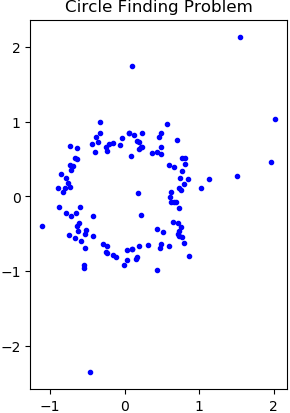
\includegraphics[width=0.6\linewidth]{./images/noisy_circle.png}
   \caption{Example of Circle Finding Problem}
   \label{fig:circle_finding}
\end{figure}


%------------------------------------------------------------------------
\section{Related Work}
\label{section:related_work}


%-------------------------------------------------------------------------
\subsection{Noisy Circle Finding Problem}

The noisy circle finding problem has been a classic exercise for computer vision students and an ongoing research topic for scholars. There are many approaches to solving this problem, including RANSAC, Patch Matching, Neural Network, etc.

For our experiment, we adopted and extended on an existing RANSAC circle detection project \cite{RansacGitHub}. The original project uses RANSAC with a twist. Instead of counting the number of inliers, the author chooses the model that has the minimum distance to all data points. We modified this part back to counting the number of inliers, and extended the class to implement the BAYSAC algorithm described in Section~\ref{section:baysac}.


%-------------------------------------------------------------------------
\subsection{BAYSAC}
\label{section:baysac}

The BAYSAC algorithm \cite{BaysacPaper} first assign all points' likelihoods to be inliers to $0.5$.
For each iteration, it updates the points' likelihoods using Equation~(\ref{eq:1}), where $P_{t}(i \in \I)$ indicates the probability of point $i$ being in the inliers set $\I$ at iteration $t$;
$P(H_{t} \subseteq \I)$ indicates the probability of the sample $H$ at iteration $t$ being a subset of the inlier set $\I$. I.e. for all points in the sample $j \in H_{t}$, $j \in \I$.

\begin{align} \label{eq:1}
   P_{t}(i \in \I)
    & =
   \begin{cases}
      \dfrac{P_{t - 1}(i \in \I) P(H_{t} \not\subseteq \I \given i \in \I)}{P(H_{t} \not\subseteq \I)}
       & i \in H_{t}
      \\
      P_{t - 1}(i \in \I)
       & i \not \in H_{t}
   \end{cases}
\end{align}

To calculate $P(H_{t} \not\subseteq \I \given i \in \I)$ and $P(H_{t} \not\subseteq \I)$, Equation~(\ref{eq:2}) and Equation~(\ref{eq:3}) are used.

\begin{align} \label{eq:2}
   P(H_{t} \not\subseteq \I)
    & = 1 - P(H_{t} \subseteq \I) \nonumber
   \\
    & = 1 - \prod^{}_{j \in H_{t}} P_{t - 1}(j \in \I)
\end{align}

\begin{align} \label{eq:3}
   P(H_{t} \not\subseteq \I \given i \in \I)
    & = 1 - P(H_{t} \subseteq \I \given i \in \I) \nonumber
   \\
    & = 1 - \prod^{}_{j \in H_{t}; j \neq i} P_{t - 1}(j \in \I) \nonumber
   \\
    & = 1 - \dfrac{P(H_{t} \subseteq \I)}{P_{t - 1}(i \in \I)}
\end{align}

Finally, combining Equations~(\ref{eq:2}, \ref{eq:3}) with Equation~(\ref{eq:1}), we derive Equation~(\ref{eq:4})

\begin{align} \label{eq:4}
   P_{t}(i \in \I)
    & =
   \begin{cases}
      \dfrac{P_{t - 1}(i \in \I) - P(H_{t} \subseteq \I)}{1 - P(H_{t} \subseteq \I)}
       & i \in H_{t}
      \\
      P_{t - 1}(i \in \I)
       & i \not \in H_{t}
   \end{cases}
\end{align}


%------------------------------------------------------------------------
\section{Experiment}

%-------------------------------------------------------------------------
\subsection{Algorithm}

Combining the two related work described in the Section~\ref{section:related_work}, the final BAYSAC algorithm can be written as Algorithm~\ref{algo:baysac}, where $dist(model, j)$ is the L2 distance defined by Equation~\ref{eq:5}.

\begin{align} \label{eq:5}
   dist(x_{c}, y_{c}, r_{c}, x_{j}, y_{j}) = | \sqrt{(x_{j} - x_{c})^{2} + (y_{j} - y_{c})^{2}} - r_{c} |
\end{align}

\begin{algorithm}
   \caption{BAYSAC($num\_iter$, $threshold$)}\label{algo:baysac}
   \begin{algorithmic}[1]
      \State $t = 0$, $\I = \{\}$
      \While{$t < num\_iter$ and $\I.size() < desired\_size$}
      \State Sample $H_{t}$ of ($n + 1$) points ordered by highest $P_{t - 1}(i \in \I)$
      \State Fit a polynomial $model$ of degree $n$.
      \If{$\forall j \in H_{t}$, $dist(model, j) < threshold$}
      \State $\I = \I \cup H_{t}$.
      \EndIf
      \State update all points' $P_{t}(i \in \I)$ base on Equation~\ref{eq:4}
      \State $t ++$
      \EndWhile
      \State\Return the fitted $model$ using all points in $\I$.
   \end{algorithmic}
\end{algorithm}


%-------------------------------------------------------------------------
\subsection{Experimental Design}

The parameters for the algorithms are the total number of datasets ($total\_num$), the circle to noise data point ratio ($ratio$), the circle points noise variance ($circle\_noise$) and the noisy points variance ($noisy\_noise$).

For each parameter setting, 10 iterations were run. For each iteration, two algorithms are run on the same set of generated data points. The analytic data are collected for each iteration and then averaged and plotted.

The analytic data collected after the experiment are percentage of inliers that were actual circle data (accuracy), runtime, the distance from the fitted model to the inliers, and the differences between the fitted circle's centers and radiuses using two algorithms.


%-------------------------------------------------------------------------
\subsection{Results}
\label{sec:results}


% ===== baseline =====
\textbf{Baseline Group}

The default parameters we set were $total\_num = 1000$, $ratio = 0.8$, $circle\_noise = 0.1$, $noisy\_noise = 1.0$. Due to the page constraint, only three pairs of results of the two algorithms are shown in Figure~\ref{fig:baseline_results}. See project repository \cite{ProjectRepo} for complete result. Observe that with the same dataset, RANSAC and BAYSAC produce very similar results with slight deviation.


% ===== total num =====
\textbf{Total Number of Data Points}

This part of the experiment tests the effect of the total number of data points. The number of data varies from 100 to 10100. For each epoch, the number of data is increased by 1000. The accuracy, runtime, distance to inliers and difference between two algorithms' fitted circles' centers and radiuses for each epoch is then plotted and shown in Figure~\ref{fig:total_num}.


% ===== ratio =====
\textbf{Circle to Noise Ratio}

This part of the experiment tests the circle to noise data point ratio. The ratio varies from 0.0 (only noise) to 1.0 (only circle). For each epoch, the ratio is increased by 0.1. The accuracy, runtime, distance to inliers and difference between two algorithms' fitted circles' centers and radiuses for each epoch is then plotted and shown in Figure~\ref{fig:ratio}.


% ===== num iter =====
\textbf{Number of Iterations}

This part of the experiment tests the number of iterations. The number of iterations varies from 2 to 40. For each epoch, the number of iterations is increased by 2. The accuracy, runtime, distance to inliers and difference between two algorithms' fitted circles' centers and radiuses for each epoch is then plotted and shown in Figure~\ref{fig:num_iter}.


% ===== circle noise =====
\textbf{Circle Noise}

This part of the experiment tests the circle noise variance. The variance of circle noise varies from 0.0 to 1.0. For each epoch, the variance is increased by 0.2. The accuracy, runtime, distance to inliers and difference between two algorithms' fitted circles' centers and radiuses for each epoch is then plotted and shown in Figure~\ref{fig:circle_noise}.


% ===== noisy noise =====
\textbf{Noisy Noise}

This part of the experiment tests the Noisy points' noise variance. The variance varies from 0.0 to 2.0. For each epoch, the variance is increased by 0.5. The accuracy, runtime, distance to inliers and difference between two algorithms' fitted circles' centers and radiuses for each epoch is then plotted and shown in Figure~\ref{fig:noisy_noise}.


% ===== baseline =====
\begin{figure}[!h]
   \centering
   \subfloat[Ransac-0]{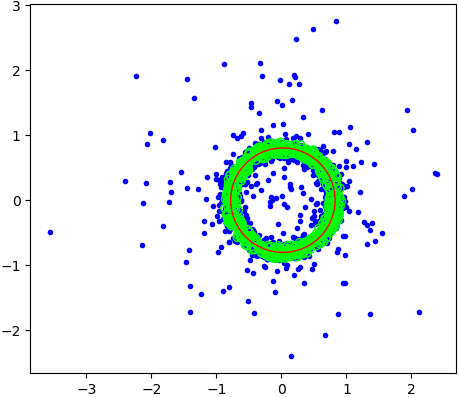
\includegraphics[width=0.23\textwidth]{images/baseline/0_ransac.png}}
   \hfill
   \subfloat[BAYSAC-0]{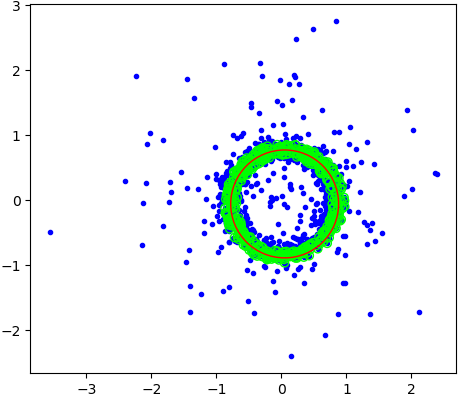
\includegraphics[width=0.23\textwidth]{images/baseline/0_baysac.png}}
   \hfill
   \subfloat[Ransac-1]{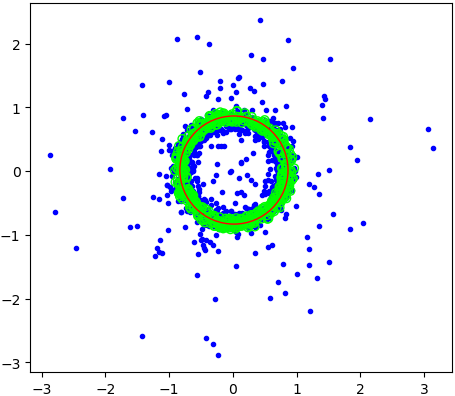
\includegraphics[width=0.23\textwidth]{images/baseline/1_ransac.png}}
   \hfill
   \subfloat[BAYSAC-1]{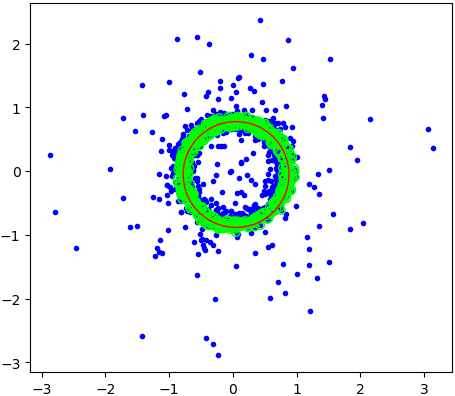
\includegraphics[width=0.23\textwidth]{images/baseline/1_baysac.png}}

   \caption{Baseline Results}
   \label{fig:baseline_results}
\end{figure}


% ===== total num =====
\begin{figure}[!h]
   \centering
   \subfloat[Accuracy]{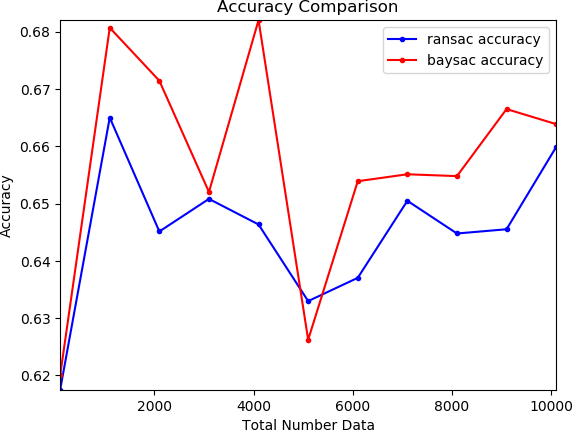
\includegraphics[width=0.23\textwidth]{images/total_num/accuracy.png}}
   \hfill
   \subfloat[Runtime]{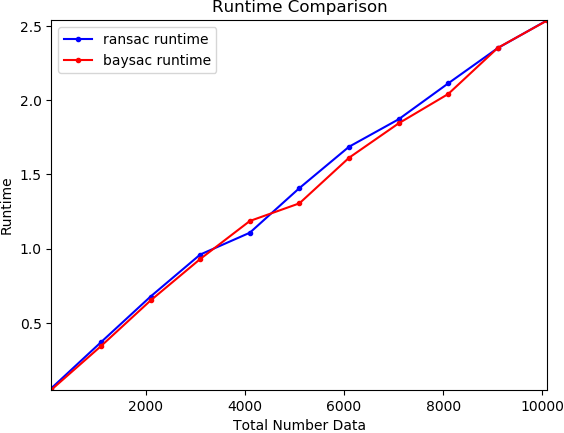
\includegraphics[width=0.23\textwidth]{images/total_num/runtime.png}}
   \\
   \subfloat[Inlier Distance]{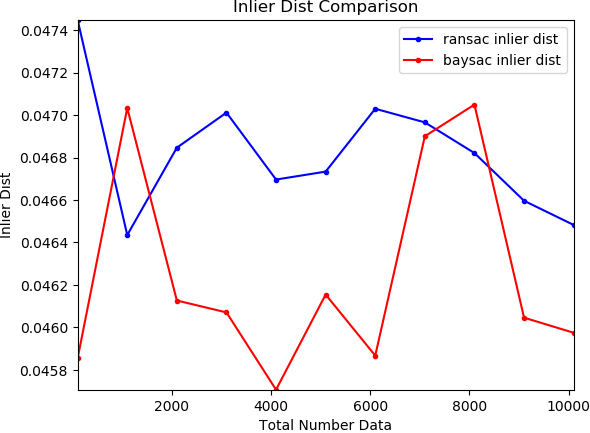
\includegraphics[width=0.23\textwidth]{images/total_num/inlier_dist.png}}
   \hfill
   \subfloat[Center and Radius Difference]{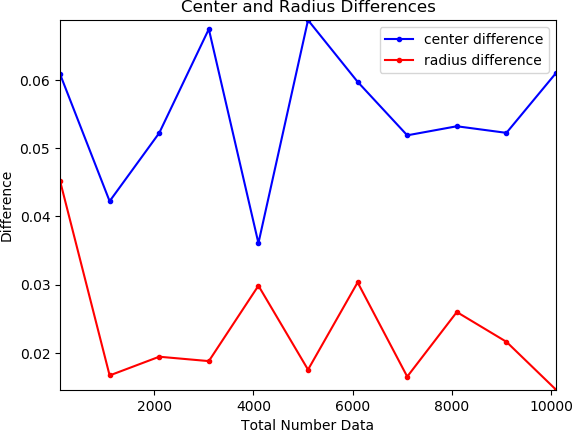
\includegraphics[width=0.23\textwidth]{images/total_num/center_radius_diff.png}}

   \caption{Total Number of Data}
   \label{fig:total_num}
\end{figure}


% ===== ratio =====
\begin{figure}[!h]
   \centering
   \subfloat[Accuracy]{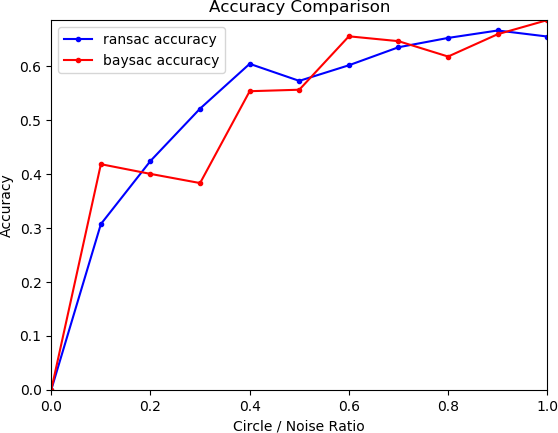
\includegraphics[width=0.23\textwidth]{images/ratio/accuracy.png}}
   \hfill
   \subfloat[Runtime]{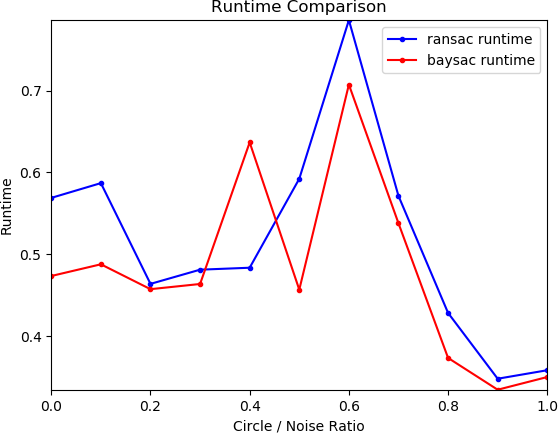
\includegraphics[width=0.23\textwidth]{images/ratio/runtime.png}}
   \\
   \subfloat[Inlier Distance]{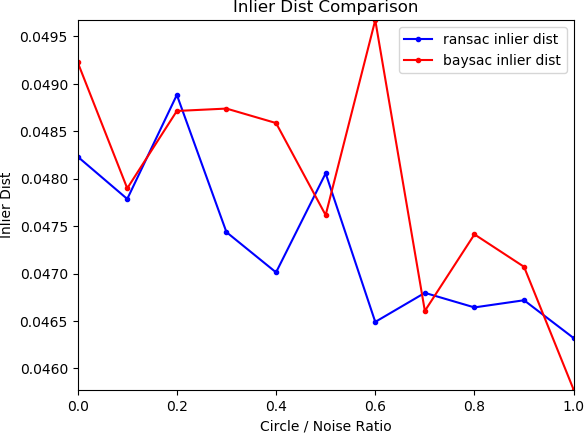
\includegraphics[width=0.23\textwidth]{images/ratio/inlier_dist.png}}
   \hfill
   \subfloat[Center and Radius Difference]{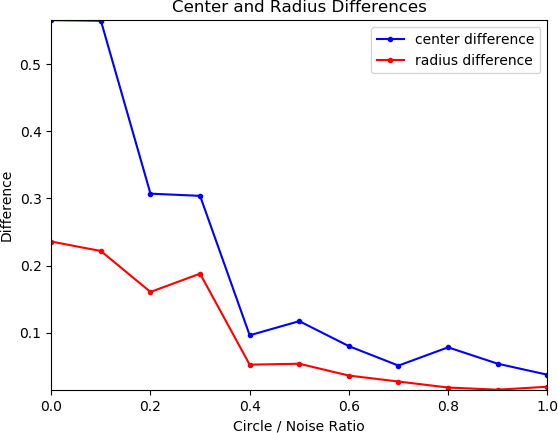
\includegraphics[width=0.23\textwidth]{images/ratio/center_radius_diff.png}}

   \caption{Circle to Noise Ratio}
   \label{fig:ratio}
\end{figure}


% ===== num iter =====
\begin{figure}[!h]
   \centering
   \subfloat[Accuracy]{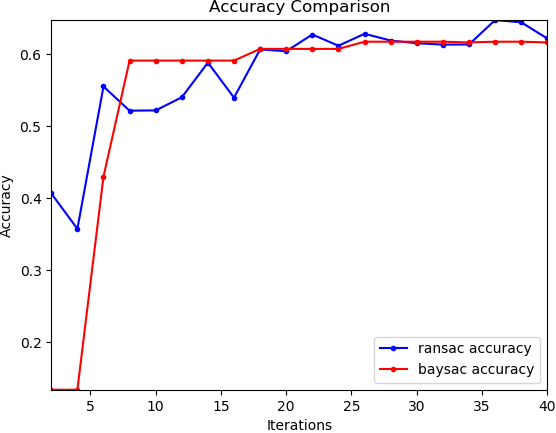
\includegraphics[width=0.23\textwidth]{images/num_iter/accuracy.png}}
   \hfill
   \subfloat[Runtime]{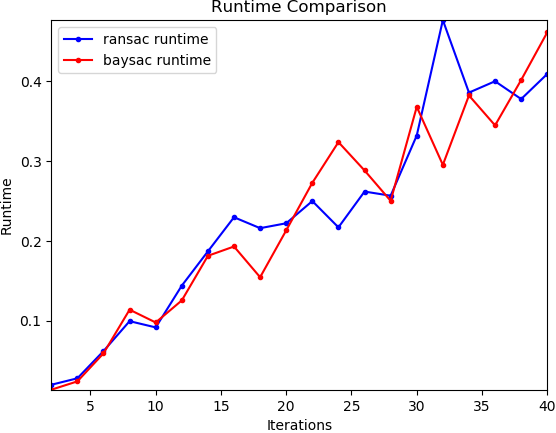
\includegraphics[width=0.23\textwidth]{images/num_iter/runtime.png}}
   \\
   \subfloat[Inlier Distance]{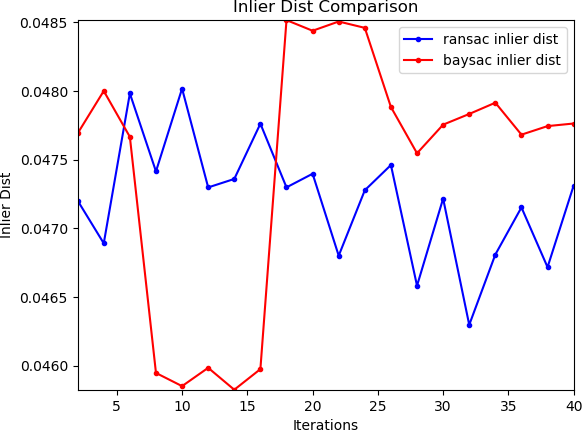
\includegraphics[width=0.23\textwidth]{images/num_iter/inlier_dist.png}}
   \hfill
   \subfloat[Center and Radius Difference]{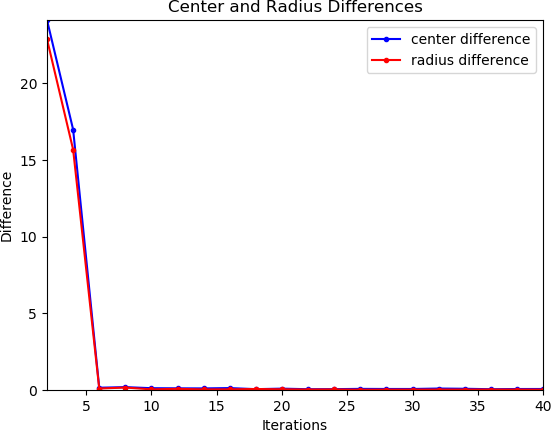
\includegraphics[width=0.23\textwidth]{images/num_iter/center_radius_diff.png}}

   \caption{Number of Iterations}
   \label{fig:num_iter}
\end{figure}


% ===== circle noise =====
\begin{figure}[!h]
   \centering
   \subfloat[Accuracy]{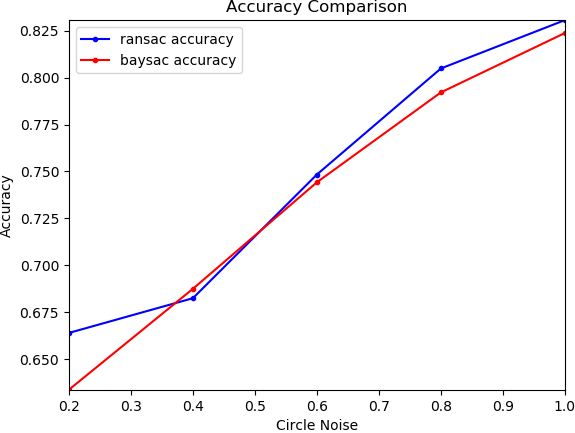
\includegraphics[width=0.23\textwidth]{images/circle_noise/accuracy.png}}
   \hfill
   \subfloat[Runtime]{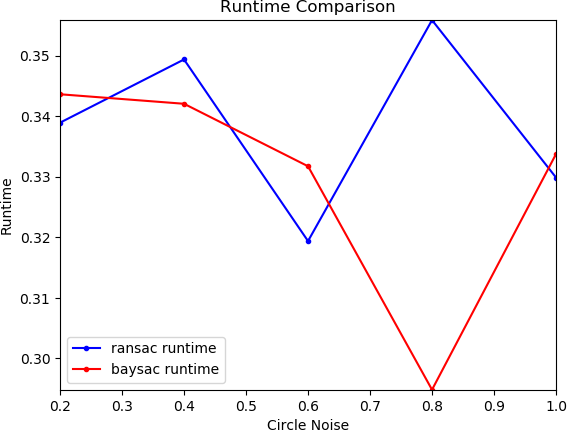
\includegraphics[width=0.23\textwidth]{images/circle_noise/runtime.png}}
   \\
   \subfloat[Inlier Distance]{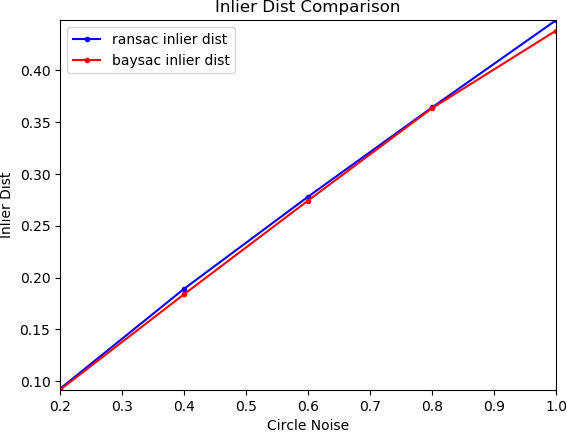
\includegraphics[width=0.23\textwidth]{images/circle_noise/inlier_dist.png}}
   \hfill
   \subfloat[Center and Radius Difference]{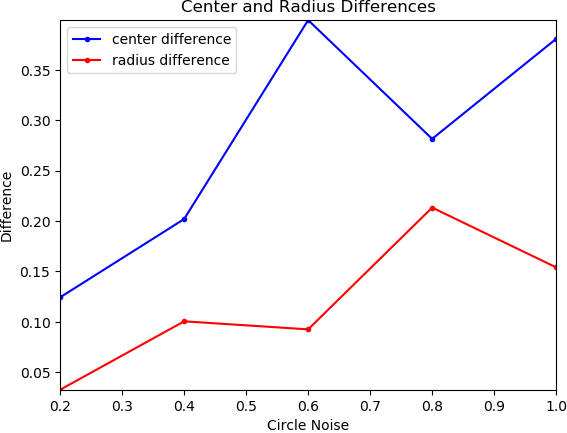
\includegraphics[width=0.23\textwidth]{images/circle_noise/center_radius_diff.png}}

   \caption{Circle Noise}
   \label{fig:circle_noise}
\end{figure}


% ===== noisy noise =====
\begin{figure}[!h]
   \centering
   \subfloat[Accuracy]{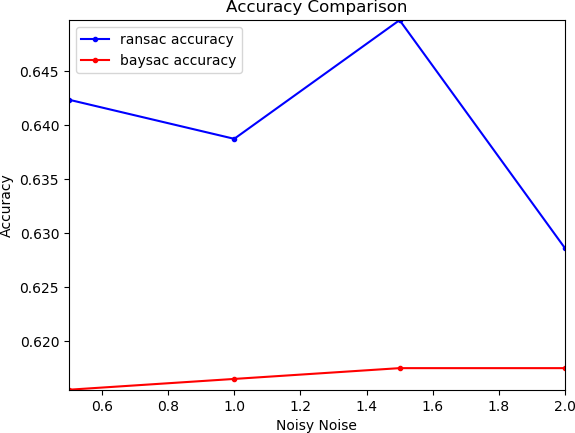
\includegraphics[width=0.23\textwidth]{images/noisy_noise/accuracy.png}\label{fig:noisy_noise_accuracy}}
   \hfill
   \subfloat[Runtime]{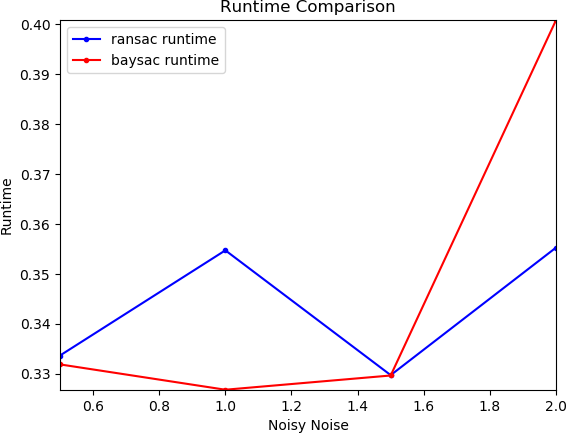
\includegraphics[width=0.23\textwidth]{images/noisy_noise/runtime.png}}
   \\
   \subfloat[Inlier Distance]{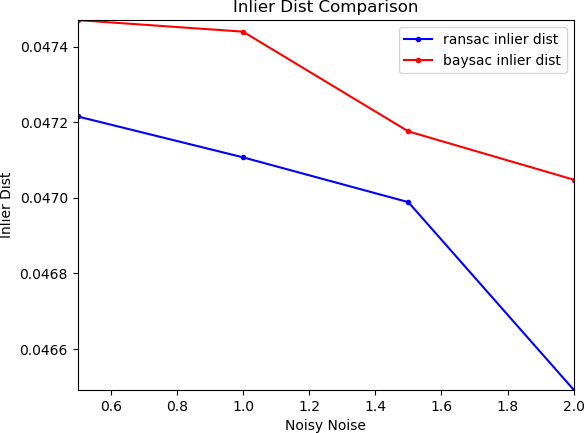
\includegraphics[width=0.23\textwidth]{images/noisy_noise/inlier_dist.png}}
   \hfill
   \subfloat[Center and Radius Difference]{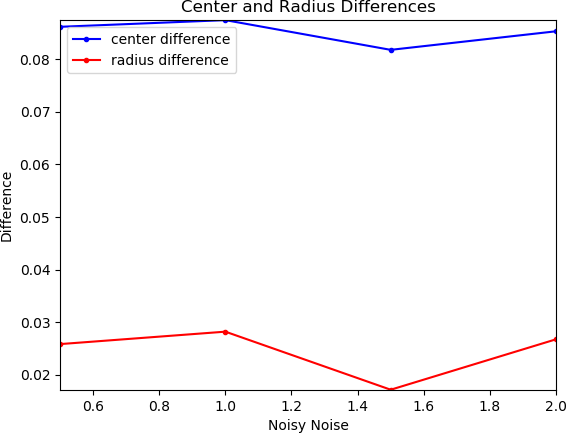
\includegraphics[width=0.23\textwidth]{images/noisy_noise/center_radius_diff.png}}

   \caption{Noisy Noise}
   \label{fig:noisy_noise}
\end{figure}

%------------------------------------------------------------------------
\section{Conclusions}

Base on the results shown in Section~\ref{sec:results}, we can see that under the problem of noisy circle detection, RANSAC and BAYSAC performs almost equally well.
The accuracies and runtimes for two the two algorithms are very similar. Note that for Figure~\ref{fig:noisy_noise_accuracy}, the y-axis scale is enlarged because the accuracies for RANSAC and BAYSAC are very similar.

By looking at the Center and Radius Differences, the results of RANSAC and BAYSAC converges as the number of iterations increases, circle to noise ratio increases (there are more circle points than random noise given the same number of total data points) and circle noise decreases.

In the original BAYSAC paper \cite{BaysacPaper}, the author claimed that BAYSAC could potentially help reduce the failure rate by up to $78\%$ compared to vanilla RANSAC. However, we were not able to show this through our experiment. One potential reason is that the noisy circle detection problem is at a very low dimension, and circle is a very low degree polynomial ($n = 2$). In the future, one possible improvement to this experiment is to compare RANSAC and BAYSAC results for solving a higher dimension problem.

%------------------------------------------------------------------------
\pagebreak
{\small
   \bibliographystyle{ieee_fullname}
   \bibliography{reportbib}
}

\end{document}
